
\section*{№ 4.26}
\begin{mdframed}
На колі радіуса $r$ навмання вибрано 2 точки. Знайти ймовірність того, що відстань між ними не більше $r$
\end{mdframed}

\begin{multicols}{2}
	$$
	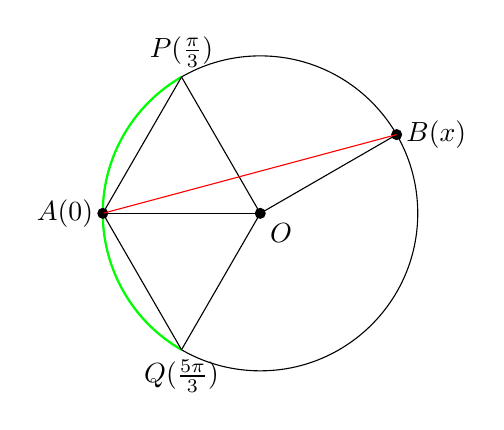
\begin{tikzpicture}
		\def\R{2};
		\coordinate (O) at (0,0);
		\path (O) ++(180:\R) coordinate (A) node[left] {$A(0)$};
		\path (O) ++(30:\R) coordinate (B) node[right] {$B(x)$};
		\path (O) ++(180-60:\R) coordinate (P) node[above] {$P(\frac{\pi}{3})$};
		\path (O) ++(180+60:\R) coordinate (Q) node[below] {$Q(\frac{5\pi}{3})$};
		% \fill[green!25] (A) -- (P) arc (180-60:180:\R);
		% \fill[green!25] (A) -- (Q) arc (180+60:180:\R);
		\fill (O) circle (2pt) node[below right] {$O$};
		\draw (O) circle[radius=\R];
		\draw[thick, green] (Q) arc (180+60:180-60:\R);
		\draw (O) -- (B);
		\draw (O) -- (A);
		\draw (O) -- (P);
		\draw (O) -- (Q);
		\fill (A) circle (2pt);
		\fill (B) circle (2pt);
		\draw[red] (A) -- (B);
		\draw (A) -- (P);
		\draw (A) -- (Q);
	\end{tikzpicture}
	$$

	\columnbreak
	
	$$
	\Omega = [-\pi, +\pi] \ni x \text{ - координата точки B}
	$$
	$$
	A = \{x \in \Omega \;|\; \overline{AB} \le r\} = [-\frac{\pi}{3}; +\frac{\pi}{3}]
	$$
	\begin{mdframed}[style=ans]
		$$
		P(A) = \frac{\mu(A)}{\mu(\Omega)} = \frac{\frac{2\pi}{3}}{2\pi} = \frac{1}{3} 
		$$
	\end{mdframed}
\end{multicols}

\section*{№ 4.27}

\begin{mdframed}
	На дiагоналi АС прямокутника ABCD зi сторонами 2см та 3см навмання 
	незалежно одна вiд одної вибрано точки E та F. 
	Знайдiть ймовiрнiсть того, що площа круга з центром в точцi E та 
	радiусом EA виявиться принаймнi втричi бiльшою за площу круга з 
	центром в точцi F та радiусом FC.
\end{mdframed}

$$
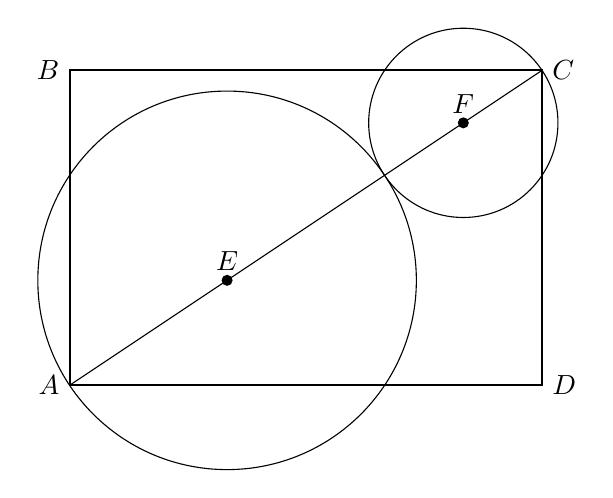
\begin{tikzpicture}
	\draw[thick] (0,0) coordinate (A) node[left] {$A$} -- 
	(0,4) coordinate (B) node[left] {$B$} -- 
	(6,4) coordinate (C) node[right] {$C$} -- 
	(6,0) coordinate (D) node[right] {$D$} -- cycle;
	\draw (A) -- (C);
	\fill (6/3,4/3) coordinate (E) node[above] {$E$} circle (2pt);
	\fill (5,5/6*4) coordinate (F) node[above] {$F$} circle (2pt);
	\draw (E) circle[radius=sqrt(36+16)/3];
	\draw (F) circle[radius=sqrt(36+16)*1/6];
\end{tikzpicture}
$$

$$
(S_E \ge 3 \cdot S_F) \iff (2\pi\overline{AE}^2 \ge 3\cdot2\pi\overline{FC}^2)
$$
Тобто 
$$
\overline{AE}^2 \ge 3 \cdot \overline{FC}^2
$$
$$
\Omega = [0;1]^2 \ni (f,e) \text{ - координати точок $F$ та $E$}
$$
$$
A = \{(f,e)\in\Omega \;|\; e^2 \ge 3 \cdot (1-f)^2 \} \implies
$$
$$
\implies |e| \ge \sqrt{3} \cdot |1-f| \implies e \ge \sqrt{3} \cdot (1-f)
$$

Зауважу, що перетин $e = \sqrt{3} (1-f)$ з $e=1$ відбувається в 
точці $(1-\frac{1}{\sqrt{3}}, 1)$.

$$\begin{tikzpicture}
	\fill[green!25] ($({3-3/sqrt(3)},3)$) coordinate (Q)
	-- (3,3) -- (3,0) -- cycle;
	\draw[thin, black!50] (0,0) grid[step=1cm] (3,3);
	\draw[thick, ->] (0,0) node[left] {$0$} -- (3,0) node[right] {$f$};
	\node[below] at (3,0) {$1$};
	\draw[thick, ->] (0,0) -- (0,3) node[above] {$e$};
	\node[left] at (0,3) {$1$};
	\draw (Q) node[above] {$1-\frac{1}{\sqrt{3}}$} -- (3,0);
	\node[right] at (2,2) {$e = \sqrt{3} (1-f)$};
	\fill (Q) circle (2pt);
	\end{tikzpicture}
$$

\begin{mdframed}[style=ans]
	$$
	P(A) = \frac{\frac{1}{2}(1-\frac{1}{\sqrt 3})\cdot 1}{1^2} 
	= \frac{1}{2}\left(1-\frac{1}{\sqrt 3}\right)
	$$
\end{mdframed}

\section*{№ 4.28}
\begin{mdframed}
	\begin{enumerate}
		\item $L_{(0,0)}(2n,0)$ при
		\subitem (a) $S_i > 0,\;i=\overline{1,2n-1}$, тобто к-сть додатніх шляхів 
		\subitem (b) $S_i \ge 0,\;i=\overline{1,2n-1}$, тобто к-сть невід'ємних шляхів 
		\item $L_{(0,m)}(2n,0)$ при
		\subitem (a) $S_i > 0,\;i=\overline{1,2n-1}$, тобто к-сть додатніх шляхів 
		\subitem (b) $S_i \ge 0,\;i=\overline{1,2n-1}$, тобто к-сть невід'ємних шляхів 
	\end{enumerate}
\end{mdframed}

\begin{mdframed}[backgroundcolor = violet!10]
	Кількість шляхів з $(0,0)$ в $(x,y)$:
	$$L_{(0, 0)}(x,y) = C_{x}^{\frac{x+y}{2}} = C_{x}^{\frac{x-y}{2}}$$
	Кількість шляхів з $(0,y0)$ в $(x,y)$, що перетинають чи дотикаються $S=0$:
	$$
	L_{(0,y0)}^{\times}(x,y) = L_{(0,-y0)}(x,y)
	$$
	Для інших випадків, можемо переносити початок координат:
	$$L_{(x_0,y_0)}(x,y) = L_{(0,0)}(x-x_0, y-y_0)$$
\end{mdframed}

Останній крок має відбутись з $(2n-1,1)$ до $(2n,0)$. 
Інакше ми йдемо з $(2n-1,-1)$ і таким чином порушимо додатність та невід'ємність шляху, 
бо тоді $S_{2n-1}<0$. 
Отже, беремо за кінцеву точку $(2n-1,1)$. 

\subsection*{1. $(0,0) \to (2n,0)$}
Одразу зауважу, що перший крок в обох випадках може бути лише \textbf{вгору}, 
бо інакше ми порушимо умови додатності та невід'ємності шляху.
Тобто розглядаємо одразу $L_{(1,1)}(2n-1,1)$

\subsubsection*{(a) $S_i > 0$}
\begin{align*}
A &= L_{(1,1)}(2n-1,1) - L^{\times}_{(1,1)}(2n-1,1) = \\
&= L_{(1,1)}(2n-1,1) - L_{(1,-1)}(2n-1,1)
= L_{(0,0)}(2n-2,0) - L_{(0,0)}(2n-2,2) = \\
&= C_{2n-2}^{n-1} - C_{2n-2}^{n} 
= \frac{(2n-2)!}{(n-1)!(n-1)!} \cdot \frac{(2n-2)!}{n!(n-2)!} =\\
&= (2n-2)! \cdot ( (n-1)!(n-1)!n!(n-2)! )^{-1} = 
(2n-2)! \cdot \left( ((n-1)!)^4 \cdot \frac{n}{n-1} \right)^{-1} = \\
&= \frac{(2n-2)!}{((n-1)!)^4} \cdot \frac{n-1}{n}
\end{align*}

\subsubsection*{(b)}
Те саме, що в (а), але тепер шлях має бути строго вищим за $S=-1$.
Відображення точки $(1,1)$ відносно $S=-1$ - це точка $(1,-3)$.
\begin{align*}
	B &= L_{(1,1)}(2n-1,1) - L^{\times S=-1}_{(1,1)}(2n-1,1) = \\
	&= L_{(1,1)}(2n-1,1) - L_{(1,-3)}(2n-1,1)
	= L_{(0,0)}(2n-2,0) - L_{(0,0)}(2n-2,4) = \\
	&= C_{2n-2}^{n-1} - C_{2n-2}^{n+1} 
\end{align*}

\begin{mdframed}[style=ans]
	$$\text{1.a)}\quad A = C_{2n-2}^{n-1} - C_{2n-2}^{n}$$
	$$\text{1.b)}\quad B = C_{2n-2}^{n-1} - C_{2n-2}^{n+1}$$
\end{mdframed}


\subsection*{2. $(0,m) \to (2n,0)$}

\subsubsection*{(a)}
\begin{align*}
A &= L_{(0,m)}(2n-1,1) - L^{\times S=0}_{(0,m)}(2n-1,1) = \\
&= L_{(0,m)}(2n-1,1) - L_{(0,-m)}(2n-1,1)
= L_{(0,0)}(2n-1,1-m) - L_{(0,0)}(2n-1,1+m) = \\
&= C_{2n-1}^{n-\frac{m}{2}} - C_{2n-1}^{n+\frac{m}{2}}
\end{align*}

\subsubsection*{(b)}
Те саме, що в (а), але тепер шлях має бути строго вищим за $S=-1$.
Відображення точки $(0,m)$ відносно $S=-1$ - це точка $(0,-m-2)$.
\begin{align*}
	B &= L_{(0,m)}(2n-1,1) - L^{\times S=-1}_{(0,m)}(2n-1,1) = \\
	&= L_{(0,m)}(2n-1,1) - L_{(0,-m-2)}(2n-1,1)
	= L_{(0,0)}(2n-1,1-m) - L_{(0,0)}(2n-1,m+3) = \\
	&= C_{2n-1}^{n-\frac{m}{2}} - C_{2n-1}^{n+\frac{m}{2}+1}
\end{align*}

\begin{mdframed}[style=ans]
	$$\text{2.a)}\quad A = C_{2n-1}^{n-\frac{m}{2}} - C_{2n-1}^{n+\frac{m}{2}}$$
	$$\text{2.b)}\quad B = C_{2n-1}^{n-\frac{m}{2}} - C_{2n-1}^{n+\frac{m}{2}+1}$$
\end{mdframed}

\section*{№ 4.29}
\begin{mdframed}
	В останнiй тур виборiв вийшли кандидати A та B. Кандидат A набрав n голосiв,
	кандидат B — m голосiв. Виборцi голусували послiдовно. Знайдiть ймовiрнiсть
	того, що кандидат A не вiдставав вiд B, якщо:
	\begin{enumerate}
		\item $n\ge m$
		\item $n = m$
	\end{enumerate}
\end{mdframed}

Розглянемо величину $S_i = n_i-m_i$.
Кандидат А не відставав від В $\iff S_i \ge 0 ,\; i = \overline{0,n+m}$
Маємо випадкове симетричне блукання на прямій з координатою $S$.
$$|\Omega| = L_{(0,0)}(n+m,n-m) = C_{n+m}^{\frac{(n+m) + (n-m)}{2}} = C_{n+m}^n$$

\begin{enumerate}
	\item $n > m \quad (\implies S_{n+m} > 0)$
	$$A = \{\text{невід'ємні шляхи}\}$$
	Шляхи невід'ємні $\implies S_1 = 1$. 
	Інакше в перший же крок порушуємо невід'ємність.
	З останнім кроком все ок.
	$$|A| = L_{(1,1)}(n+m,n-m) - L^{\times S=-1}_{(1,1)}(n+m,n-m) = $$
	$$= |\Omega| - L_{(1,-3)}(n+m,n-m) = |\Omega| - L_{(0,0)}(n+m-1,n-m+3) = $$
	$$= |\Omega| - C_{n+m-1}^{\frac{n+m-1+n-m+3}{2}} = 
	|\Omega| - C_{n+m-1}^{n+1}$$

	\begin{align*}
		P(A) &= \frac{|\Omega| - C_{n+m-1}^{n+1}}{|\Omega|} = 1 - \frac{C_{n+m-1}^{n+1}}{C_{n+m}^n} = \\
		&= 1 - \frac{(n+m-1)!}{(n+m)!} \cdot \frac{n!m!}{(n+1)!(m-2)!} 
		= 1 - \frac{1}{n+m} \cdot \frac{m(m-1)}{n+1} = 1 - \frac{m(m-1)}{(n+m)(n+1)}
	\end{align*}

	\item $n = m \quad(\implies S_{n+m} = 0)$
	
	Все те саме, що й в \textbf{1}, але інший останній крок - 
	тепер він може бути лише з $(n+m-1, 1)$ до $(n+m,0)$. 
	Інакше він з $(n+m-1, -1)$ , тобто порушується невід'ємність шляху.

	$$B = \{\text{невід'ємні шляхи}\}$$
	Шляхи невід'ємні $\implies S_1 = 1\;\wedge\;S_{n+m-1} = 1$. 
	Інакше порушуємо невід'ємність.
	
	$$|B| = L_{(1,1)}(n+m-1,n-m-1) - L^{\times S=-1}_{(1,1)}(n+m-1,n-m-1) = $$
	$$= |\Omega| - L_{(1,-3)}(n+m-1,n-m-1) = |\Omega| - L_{(0,0)}(n+m-2,n-m+2) = $$
	$$= |\Omega| - C_{n+m-2}^{\frac{n+m-2+n-m+2}{2}} = 
	|\Omega| - C_{n+m-2}^{n}$$

	\begin{align*}
		P(B) &= \frac{|\Omega| - C_{n+m-2}^{n}}{|\Omega|} = 1 - \frac{C_{n+m-2}^{n}}{C_{n+m}^n} = \\
		&= 1 - \frac{(n+m-2)!}{(n+m)!} \cdot \frac{n!m!}{n!(m-2)!} 
		= 1 - \frac{1}{(n+m)(n+m-1)} \cdot m(m-1) =\\
		&= 1 - \frac{m(m-1)}{(n+m)(n+m-1)}
	\end{align*}
\end{enumerate}

\begin{mdframed}[style=ans]
	$$\textbf{1.}\; P(A) = 1 - \frac{C_{n+m-1}^{n+1}}{C_{n+m}^n} = 1 - \frac{m(m-1)}{(n+m)(n+1)}$$
	$$\textbf{2.}\; P(B) = 1 - \frac{C_{n+m-2}^{n}}{C_{n+m}^n} = 1 - \frac{m(m-1)}{(n+m)(n+m-1)}$$
\end{mdframed}

\section*{№ 4.30}
\begin{mdframed}
У буфетi продаються пирiжки вартiстю 50 коп. Бiля буфету зiбралося m + n
студентiв, причому n з них мають монети по 50 коп., а решта m мають лише
по однiй гривнi (m ≤ n). Знайдiть ймовiрнiсть того, що жодному студентовi не
доведеться чекати решти, якщо на початку роботи в касi 
\textbf{було $p$ монет по 50 коп.}
\end{mdframed}

Вводимо величину $S_i = p + n_i - m_i \ge 0$, де 
$n_i$ - кількість обслужених студентів із 50 коп. (тобто без решти), 
$m_i$ - кількість обслужених студентів із 1 грн. (тобто тих, кому була потрібна решта).

Тобто $S_i$ - кількість копійок на i-тому кроці.

Зауважу, що в кінці обслуговування залишиться 
$S_{n+m} = p + n - m$ копійок по 50коп. 
Через це можна не виділяти ситуацію, коли $n=m$: 
останній крок ніколи не буде з $S_{n+m-1}<0$. 

$$|\Omega| = L_{(0,p)}(n+m, p+n-m) = C_{n+m}^n$$

$$|A| = |\Omega| - L^{\times (S=-1)}_{(0,p)}(n+m, p+n-m)
= |\Omega| - L_{(0,-p-2)}(n+m,p+n-m) =$$
$$= |\Omega| - C_{n+m}^{\frac{n+m+n-m+2p+2}{2}} = 
|\Omega| - C_{n+m}^{n+p+1}$$
\begin{mdframed}[style=ans]
$$P(A) = \frac{|\Omega| - C_{n+m}^{n+p+1}}{|\Omega|} = 
1 - \frac{C_{n+m}^{n+p+1}}{C_{n+m}^n}$$
\end{mdframed}

\section*{№ 4.31}
\begin{mdframed}
	Частинка здiйснює симетричне випадкове блукання на прямiй. В початковий
	момент часу вона знаходилася у точцi з координатою 4 i через шiсть крокiв знову
	опинилася в цiй точцi.Знайдiть ймовiрнiсть того, що це було перше повернення
	у вихiдну точку
\end{mdframed}

Спочатку, зсунемо початок відліку в 4. 
Тобто тепер починаємо в точці $0$ та повертаємось в неї ж через 6 кроків.

$$
\begin{tikzpicture}
	\draw[thin, black!50] (0,-3) grid[step=0.5cm] (5,3);
	\draw[thick, ->] (0,-3) -- (0,3) coordinate (A);
	\node[above] at (A) {$S$};
	\node[left] at (A) {$6$};
	\draw[thick, ->] (0,0) node[left] {$0$} -- (5,0) coordinate (B);
	\node[right] at (B) {$i$};
	\node[above] at (3,3) {$i=6$};
	
	\draw[dashed] (3,-3) -- (3,3);
	\draw[dashed] (0,0.5) -- (5,0.5) node[right] {$S=1$};
	\draw[dashed] (0,-0.5) -- (5,-0.5) node[right] {$S=-1$};

	\draw[dashed] (0,0) -- (1.5,1.5) -- (3,0);
	\draw[dashed] (0,0) -- (1.5,-1.5) -- (3,0);

	\draw[blue] (0,0) -- ($0.5*(1,1)$) -- ($0.5*(2,2)$) -- ($0.5*(3,1)$) -- ($0.5*(4,2)$) -- ($0.5*(5,1)$) -- (3,0);
	\draw[violet] (0,0) -- ($0.5*(1,-1)$) -- (1,-1) -- (1.5,-0.5) -- (2,-1) -- ($0.5*(5,-1)$) -- ($0.5*(6,0)$);
	\fill ($0.5*(1,1)$) circle (2pt);
	\fill ($0.5*(5,1)$) circle (2pt);
	\fill ($0.5*(1,-1)$) circle (2pt);
	\fill ($0.5*(5,-1)$) circle (2pt);
	\fill ($0.5*(6,0)$) circle (2pt);
	\fill ($0.5*(2,2)$) circle (2pt);
	\fill ($0.5*(2,-2)$) circle (2pt);
	\fill ($0.5*(4,2)$) circle (2pt);
	\fill ($0.5*(4,-2)$) circle (2pt);
	\fill (0,0) circle (2pt);
\end{tikzpicture}
$$

$$
|\Omega| = L_{(0,0)}(6,0) = C_6^3 = \frac{6!}{3!3!} = 20
$$

$$
|A| = 2 \cdot L_{(1,1)}^{\ge 1}(5,1) 
= 2 L_{(2,2)}(4,2) = 2 C_2^1 = 4
$$

\begin{mdframed}[style=ans]
	$$P(A) = \frac{4}{20} = \frac{1}{5}$$
\end{mdframed}

\section*{№ 4.32}
\begin{mdframed}
	Футбольний матч мiж командами "Рисаки" i "Мустанги" закiнчився з рахунком 
	5:3 на користь "Рисакiв". 
	Знайдiть ймовiрнiсть того, що пiсля рахунку 1:1,
	який встановився на 20-iй хвилинi матчу, "Рисаки" весь час вели в рахунку.
\end{mdframed}

Рахуємо кількість голів кожної команди після кожного гола:
Нехай $n_i$ - кількість голів, яку після $i$-го гола забили Рисаки;
$m_i$ - кількість голів, яку після $i$-го гола забили Мустанги.
$i = \overline{1,m+n} = \overline{1,8}$

Вводимо величину $S_i = n_i - m_i$.
$$S_2 = 0$$
$$S_{5+3} = S_8 = 2 = 5-3$$

Рисаки весь час вели $\iff m_i > n_i \; \forall i>2$
$$A = \{{S_i} \in \Omega\;|\;\forall i>2:\;S_i > 0\}$$

$$
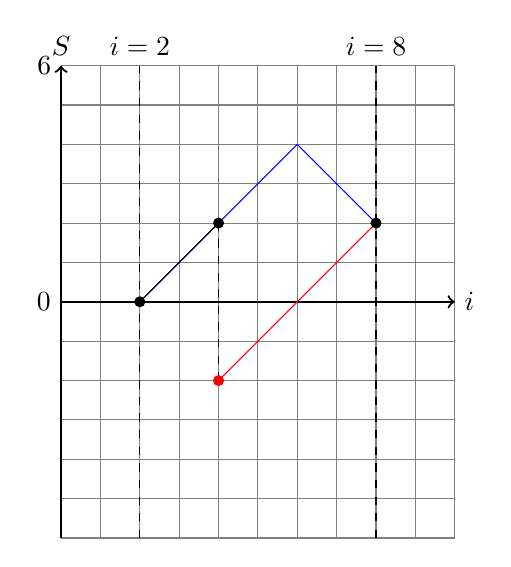
\begin{tikzpicture}
	\draw[thin, black!50] (0,-3) grid[step=0.5cm] (5,3);
	\draw[thick, ->] (0,-3) -- (0,3) coordinate (A);
	\node[above] at (A) {$S$};
	\node[left] at (A) {$6$};
	\draw[thick, ->] (0,0) node[left] {$0$} -- (5,0) coordinate (B);
	\node[right] at (B) {$i$};

	\draw[dashed] (1,-3) -- (1,3) node[above] {$i = 2$}; 
	\draw[dashed] (4,-3) -- (4,3) node[above] {$i = 8$}; 

	\draw[blue] (1,0) -- (1.5,0.5) -- (2,1) -- (3,2) -- (4,1);
	\draw (1,0) -- (2,1);
	\draw[red] (2,-1) -- (4,1);
	\draw[dashed] (2,-1) -- (2,1);

	% \fill ($0.5*(1,1)$) circle (2pt);
	% \fill ($0.5*(5,1)$) circle (2pt);
	% \fill ($0.5*(1,-1)$) circle (2pt);
	% \fill ($0.5*(5,-1)$) circle (2pt);
	% \fill ($0.5*(6,0)$) circle (2pt);
	% \fill ($0.5*(2,2)$) circle (2pt);
	% \fill ($0.5*(2,-2)$) circle (2pt);
	% \fill ($0.5*(4,2)$) circle (2pt);
	% \fill ($0.5*(4,-2)$) circle (2pt);
	\fill (1,0) circle (2pt);
	\fill (2,1) circle (2pt);
	\fill (4,1) circle (2pt);
	\fill[red] (2,-1) circle (2pt);
\end{tikzpicture}
$$

$$|\Omega| = L_{(2,0)}(8,2) = C_6^4 = \frac{6\cdot 5}{2} = 15$$
$$|A| = L^{>0}_{(2,0)}(8,2) 
= L^{>0}_{(4,2)}(8,2) = L_{(4,2)}(8,2) - L_{(4,-2)}(8,2) = $$
$$= C_4^2 - C_4^4 = \frac{4 \cdot 3 }{2} - 1 = 5$$
\begin{mdframed}[style=ans]
	$$P(A) = \frac{5}{15} = \frac{1}{3}$$
\end{mdframed}